\section{Linear Road}
\frame{\sectionpage}

\begin{frame}{Linear Road}
    \begin{figure}
        \centering
        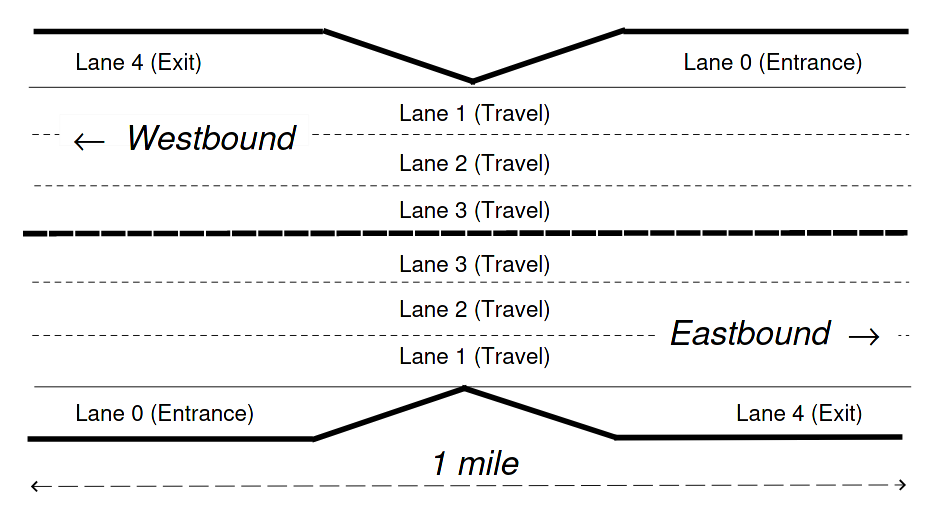
\includegraphics[scale=0.4]{lr.png}\\
        \caption{An Example Expressway Segment}
        \label{fig:lr_ex}
    \end{figure}
\end{frame}

\begin{frame}[fragile]{Query to execute}
    \begin{lstlisting}[language=SQL, caption= SEGTOLL linear road query]
        SELECT car_id, exp_way, dir, seg
        FROM CarSegStr [PARTITION BY car_id ROWS 1], CurActiveCars
        WHERE CarSegStr.car_id = CurActiveCars.car_id;
        
        SELECT exp_way, dir, seg, AVG(speed) as speed,
        FROM CarSegStr [RANGE 5 MINUTES]
        GROUP BY exp_way, dir, seg;
        
        SELECT exp_way, dir, seg, COUNT(*) as volume
        FROM CurCarSeg
        GROUP BY exp_way, dir, seg;

        SELECT S.exp_way, S.dir, S.seg, basetoll*(V.volume-150)*(V.volume-150)
        FROM SegAvgSpeed as S, SegVol as V
        WHERE S.exp_way = V.exp_way and S.dir = V.dir and S.seg = V.seg
              and S.speed <= 40;
    \end{lstlisting}
\end{frame}
